% !TEX root = main.tex
\chapter{Concept Design}
\label{chap:conceptdesign}

  The following contains the conceptual design of a rear wing based on the previous chapters. First, a walkthrough of different airfoil profiles and their benefits is followed by selection of one particular. Second, analyzing the amount of elements the wing should consists of with regards to production time and ease of construction. Third, the dimensional requirements outlined by the competition rules are given, and finally, a Product Design Specifiation (PDS) is set up to make sure that the design solution addresses all the problems it attempts to solve. Based on the PDS, an initial design is proposed, followed by a section describing the various possible methods of optimization.

  \section{Comparison of Airfoils}

    Finding a fitting airfoil requires deep investigation of airfoil databases and articles. The requirements for this airfoil according to the PDS is a really high lift wing, operating at large ranges of Reynolds numbers, where the highest (according to track regulations) is around:
    \begin{align}
      \text{Re} &= \frac{uL}{\nu} = \frac{\SI{30.56}{\metre\per\second}\SI{0.6}{\metre}}{\SI{1.491E-5}{\metre\squared\per\second}} \approx \SI{1.2E6}{}
      \intertext{to around:}
      \text{Re} &\approx \SI{3E5}{} ~\text{at}~ \SI{15}{\metre\per\second}
    \end{align}
    which is the speed estimated for the tightest corners in the competition \cite{FSrules18}. Thereto, the wanted airfoil should have soft stall characteristics, and be very resilient to laminar separation bubbles (LSB for short. The interested reader is refered to reference \cite{jkatz}). This is done by having a large leading edge radius.

    \begin{figure}
      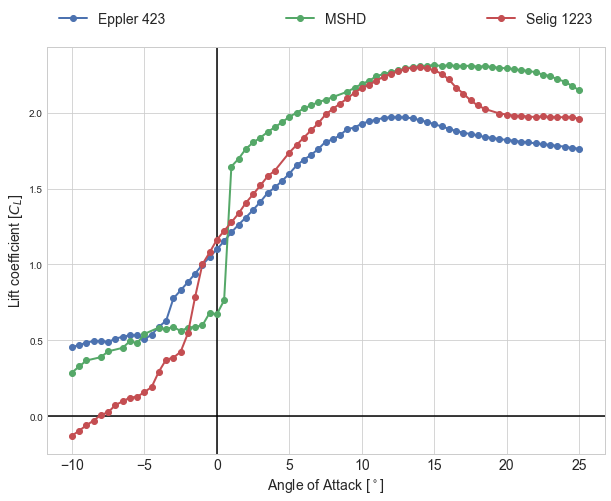
\includegraphics[width=\textwidth]{clperAOAtheory}
      \caption{A comparison of the three airfoils as a function of angle of attack. The MSHD profile shows high lifting characteristics over a wide range of angles of attack. Comparisons are from XFOIL at $\text{Re} = \SI{3E5}{}$.}
      \label{fig:AOAofairfoils}
    \end{figure}

    After a thorough research comparing high lift-low Reynolds number airfoils functioning over a wide variety of angles of attack, three airfoil are selected for further examination. The Eppler E423, the Motor Sport High Downforce (MSHD) and finally the Selig S1223. The lift coefficient can be seen as a function of angle of attack in figure \ref{fig:AOAofairfoils}.

    The MSHD performs incredibly well over a wide range of AOAs, with very low variation in lift coefficients. The MSHD airfoil is designed specifically for the Formula Student competition, which does make the choice rather obvious. The MSHD is selected for further investigation, and will be the airfoil of choice.

    Lastly, finding the right amount of elements depends on the airfoil, and based on the MSHD profile and previous studies, two elements were chosen: A main element and a scaled down flap with $35\%$ of the length of the main element \cite{winginitialangle}. The two elements will have an identical airfoil, as this is a classical way of generating successful multi element wings \cite{sameairfoilgoodidea}. This makes production time shorter, monetary cost lower and (hopefully) provides ample lift for the first generation race car.

  \section{Dimensional Requirements}

    The formula student competition has a clear ruleset dictating the dimensional requirements of aerodynamic devices. The most crucial elements are outlined below:

    \begin{tcolorbox}[colframe=seapurple,colback=seapurple!1]
      Height Restrictions:
      \begin{itemize}
        \item[T7.3.1] All aerodynamic devices rearward of a vertical plane through the rearmost portion of the front face of the driver head restraint support, excluding any padding, set to its most rearward position must be lower than $\SI{1.2}{\metre}$ from the ground.
      \end{itemize}

      Width Restrictions:
      \begin{itemize}
       \item [T7.3.2] All aerodynamic devices higher than 500 mm from the ground, must not extend outboard of the most inboard point of the rear wheel/tire.
      \end{itemize}

      Length Restrictions:
      \begin{itemize}
        \item [T7.3.3] All aerodynamic devices must not extend further rearward than 250 mm from the rearmost part of the rear tires
      \end{itemize}

      Minimum Edge Radii of Aerodynamic Devices:
      \begin{itemize}
        \item[T7.4\hphantom{.0}] All forward facing edges of aerodynamic devices that could contact a pedestrian must have a
      minimum radius of $\SI{5}{\milli\metre}$for all horizontal edges and 3 mm for vertical edges.
      \end{itemize}
      \vspace{5pt}
      \hspace*{\fill}\tiny{Rules from Formula Student UK 2018 ruleset \cite{FSrules18}.}
    \end{tcolorbox}

    The dimensional requirements from the rules was sketched on the front plane of the car's CAD drawing. This allows positioning the wing in the square seen in figure \ref{fig:cadplacement}.

    \begin{figure}
      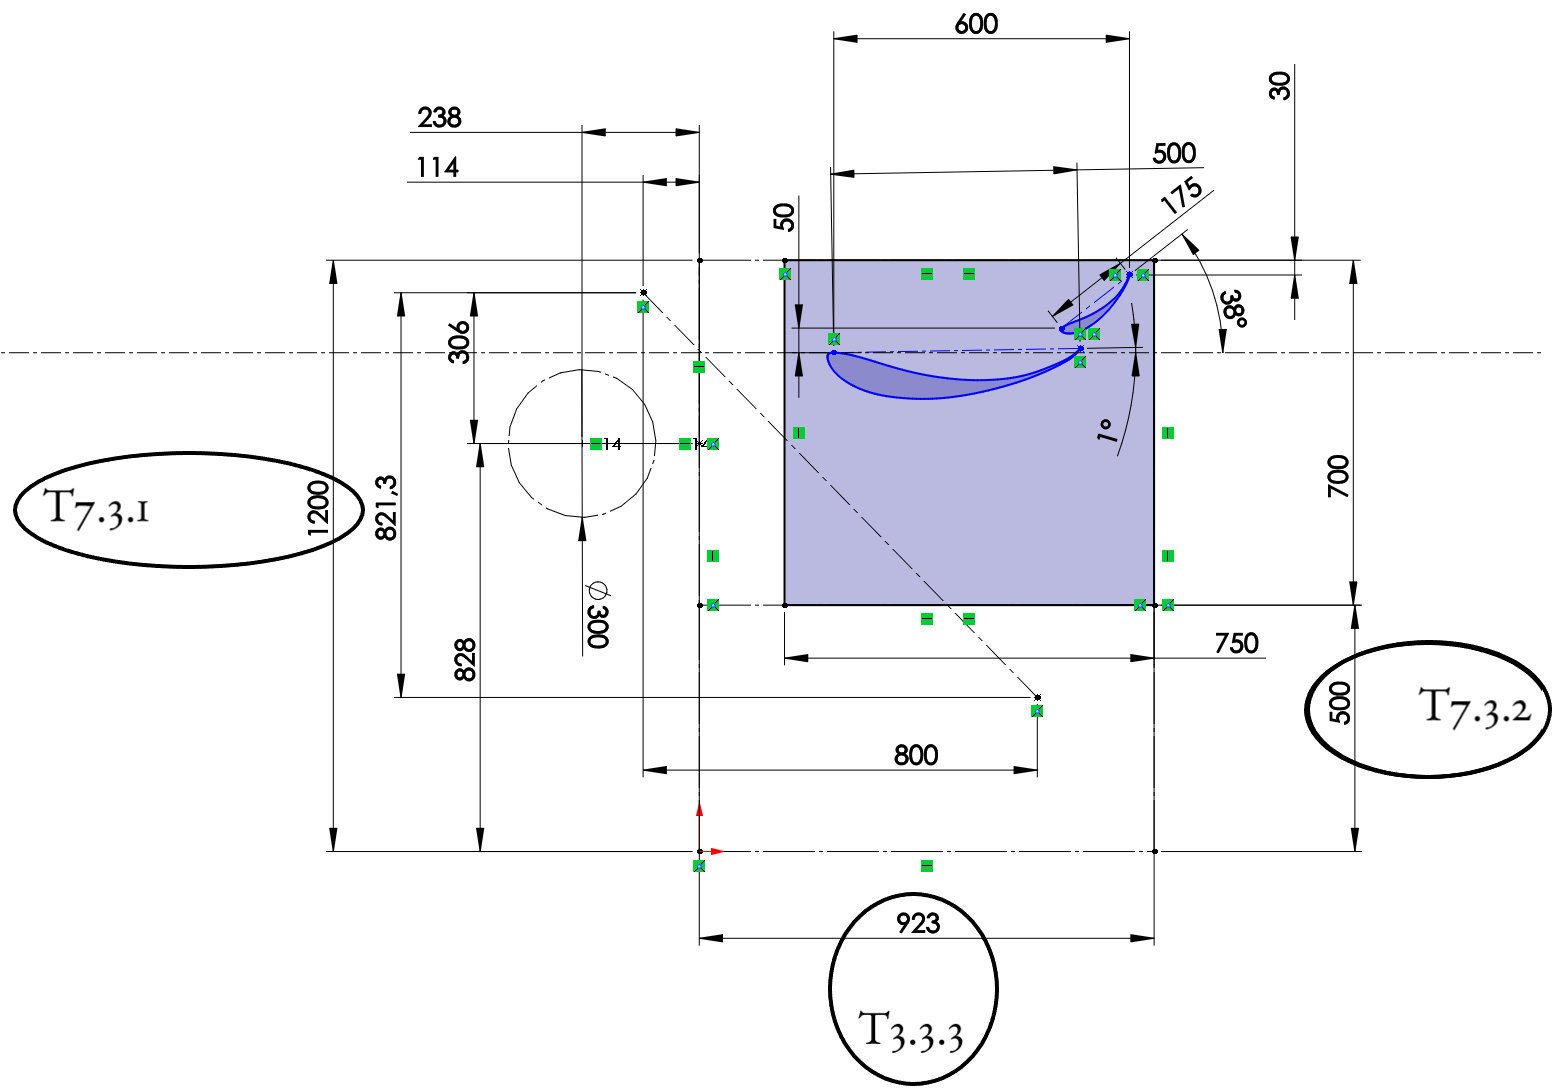
\includegraphics[width=\textwidth]{cadplacementwrules}
      \caption{The ruleset above drawn against the design of the car. The marked square is the area where the wing can be freely placed.}
      \label{fig:cadplacement}
    \end{figure}

  \section{Product Design Specification (PDS)}
  \label{sec:PDS}

    The PDS is a design tool created to ensure that the project solves the problems it set out to. The specifications uncovered in the previous sections are boiled down to their bare essentials, and in order to cover as large a solution space as possible, the PDS contains as few \emph{requirements} as possible. However, fulfilling the requirements is essential for a proper solution. While the criteria are not crucial, the criteria are the difference between an acceptable solution and a good one. The PDS will be revised at the discussion section, in order to verify the design solution fulfills all requirements.
    \begin{table}
      \begin{tabularx}{\textwidth}[t]{>{\columncolor{seapurple!40}}l XX}
      \arrayrulecolor{seapurple}\hline
      \rowcolor{white}
      \textbf{\textcolor{seapurple}{Issue}} & \textbf{\textcolor{seapurple}{Requirement}} & \textbf{\textcolor{seapurple}{Criteria}}\\
      \hline
      Weight & Must not move CM above halfway point & As low as possible \\
      Safety & Must be in compliance with FSAE rules & Should not make handling difficult for driver\\
      Durability & Must have no fatigue limit. Must to be waterproof & \\
      Performance & High downforce \& soft stall characteristic at all speeds & Should retain perfomance despite tripping. Should have end plates.\\
      Dimensioning & Must be within area defined by FSAE rules & Should allow space for motor removal. \\
      Production & Low time- and monetary cost & \\
      \end{tabularx}
      \caption{The PDS table shows how the final design lives up to the proposed specifications.}
    \end{table}
  \section{Initial Design}

    \begin{figure}
      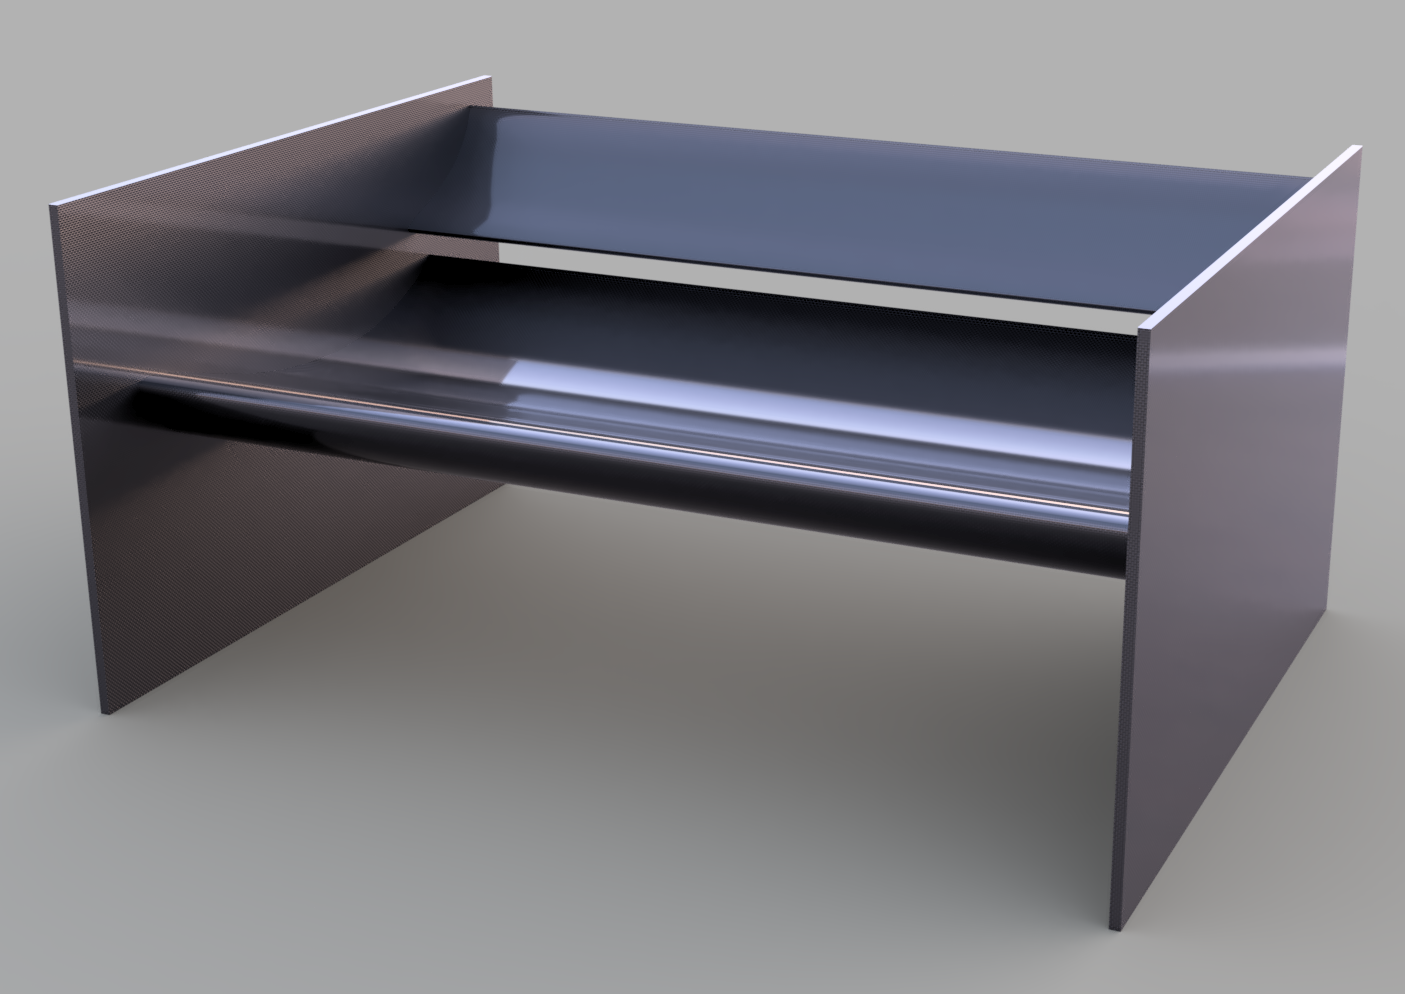
\includegraphics[width=\textwidth]{mshdinitialdesign}
      \caption{Initial design of the rear wing based on the PDS and initial research. Optimization of the wing is the next step.}
      \label{fig:firstdraftwing}
    \end{figure}

    An initial design can be made based on the PDS and the design ideas above. The MSHD airfoil has a lot of the wanted characteristics: High downforce, both leading- and trailing edge stalls are soft, and the usable AOA-ranges are high. Furthermore, based on equation \ref{eq:endplates}, we want as large end plates as possible, which will therefore fill the entirety of the allowed area. The dimensional restrictions from the competition are shown in figure \ref{fig:cadplacement}. Finally, two elements are chosen as that gives a large amount of lift over even higher angles of attack, while being cheap timewise to construct.

    A first draft of the design can be seen in \ref{fig:firstdraftwing}. As the wing is intended to be optimized, a few initial assumptions were made. The first element's tail is angled $1^\circ$ below horizontal, and the angle between the two wing elements is $36^\circ$ based on a previous study \cite{winginitialangle}. The same article provides a first guess of the relative size of the two elements, which should be a good start for the optimization process.

  \section{Optimization Tools}

    In order to optimize a design, there is three ways usually employed in aerodynamics.

    Road testing might seem the easiest method of testing, but constructing full-scale rear wing and iterating is very time consuming. Furthermore, in order to measure downforce correctly, suspension vibration, varying weather and such have to be taken into account, and as is the first car that's being produced, there is no car to test on. Lastly, the driver performance is rarely repeatable, thus making actual road testing a time consuming and inaccurate method of testing the wings.

    Wind tunnels is another option. This allows for construction of down-scaled models, as long as Reynolds numbers are scaled accordingly. However, models can also be difficult to produce, and might not reproduce full scale results correctly. Full scale testing is expensive and wind tunnels of that size are rare.

    Lastly, computational fluid dynamics offer a method of testing a wing without actually producing anything physically. Albeit the seemingly great possibilities, computer time is also expensive, and high resolution solutions require very powerful computers \cite{jkatz}. Luckily for us, we have access to the Niflheim Linux supercomputer cluster located at the Department of Physics at the Technical University of Denmark. The supercomputer has a total of 11368 CPU cores, with 235 Teraflops of processing power.

    In order to verify the numerical models applied to the problem, a wind tunnel test will be performed on a 1/4 scale model and be compared to simulations. Post verification, numerical optimization of the wing will follow in Star-CCM+.
